%!TEX root = report.tex

\chapter{Prototyp Implementierung}
\label{cha:implementierung}
In der Referenzimplementierung von \dg wird die ANTLR Syntax zur formalen Definition unserer Sprache verwendet. Darauf aufbauend wird der von ANTLR bereitgestellte Parser und Lexer genutzt, um das in \dg geschriebene Spiel zu erfassen.\\

\begin{figure}[ht]
	\centering
	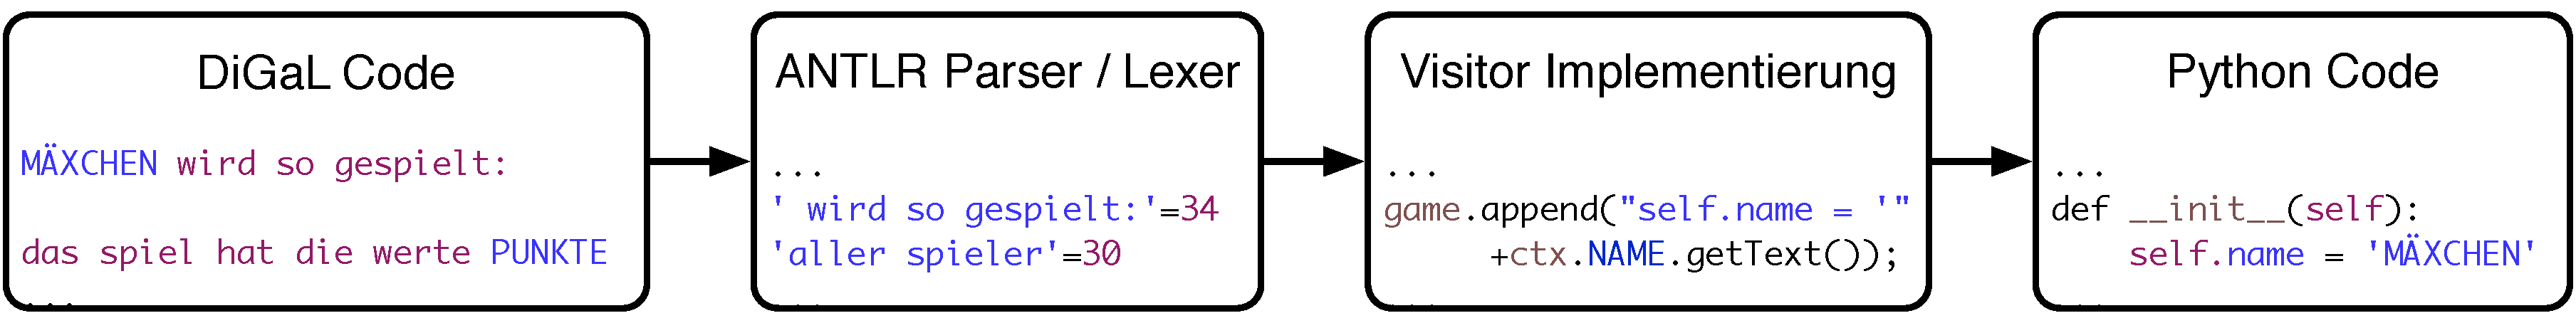
\includegraphics[width=\textwidth]{Flow.pdf}
	\caption{Ablauf der Kompilation eines DiGaL Programmes}
	\label{flow}
\end{figure}

Um sicherzustellen, dass die mit \dg geschriebenen Spiele portabel sind, wurde zum Ziel gesetzt möglichst wenige Abhängigkeiten vorauszusetzen. Ein Kriterium war dabei, dass die Ausführung des Codes nur mit der Standardbibliothek einer Zielsprache funktioniert. Daher wurde sich für eine Kompilation der Sprache entschieden, und darauf versichtet für den Endanwender auf die Installation von ANTLR vorauszusetzen. Als Zielsprache dient Python, das Syntaktisch kompakt zu programmieren ist und inhärente Konzepte unserer Sprache unterstützt (Objektorientiertheit, Funktionale Programmierung).

Zur Generierung des Python Codes wird das Visitorpattern entschieden verwendet. Die Entscheidung gründet auf die Simplizität einer Implementierung dieses Patterns, das uns als lernende ANTLR Spielentwickler nur noch abverlangt die vorgegebenen Methoden zu implementieren und uns so auf das wesentliche zu konzentrieren. 

\section{Python Framework}
\label{sec:python_framework}
	Zusammen mit der Definition der Grammatik wurden generische Methoden ausgearbeitet. Die vorhanden Methoden lassen sich in zwei Klassen differenzieren: Generische Methoden, die in vielen Würfelspielen verwendet werden; Methoden die zur Interaktion mit den Mitspielern und zur Repräsentation von Daten gegenüber diesen nötig sind. Die zweite Gruppe ergibt sich nicht aus der Domäne selbst, sondern folgt aus der nötigen Mensch-Maschine Kommunikation (Ausgaben auf der Kommandozeile).

    \begin{figure}[ht]
    	\centering
        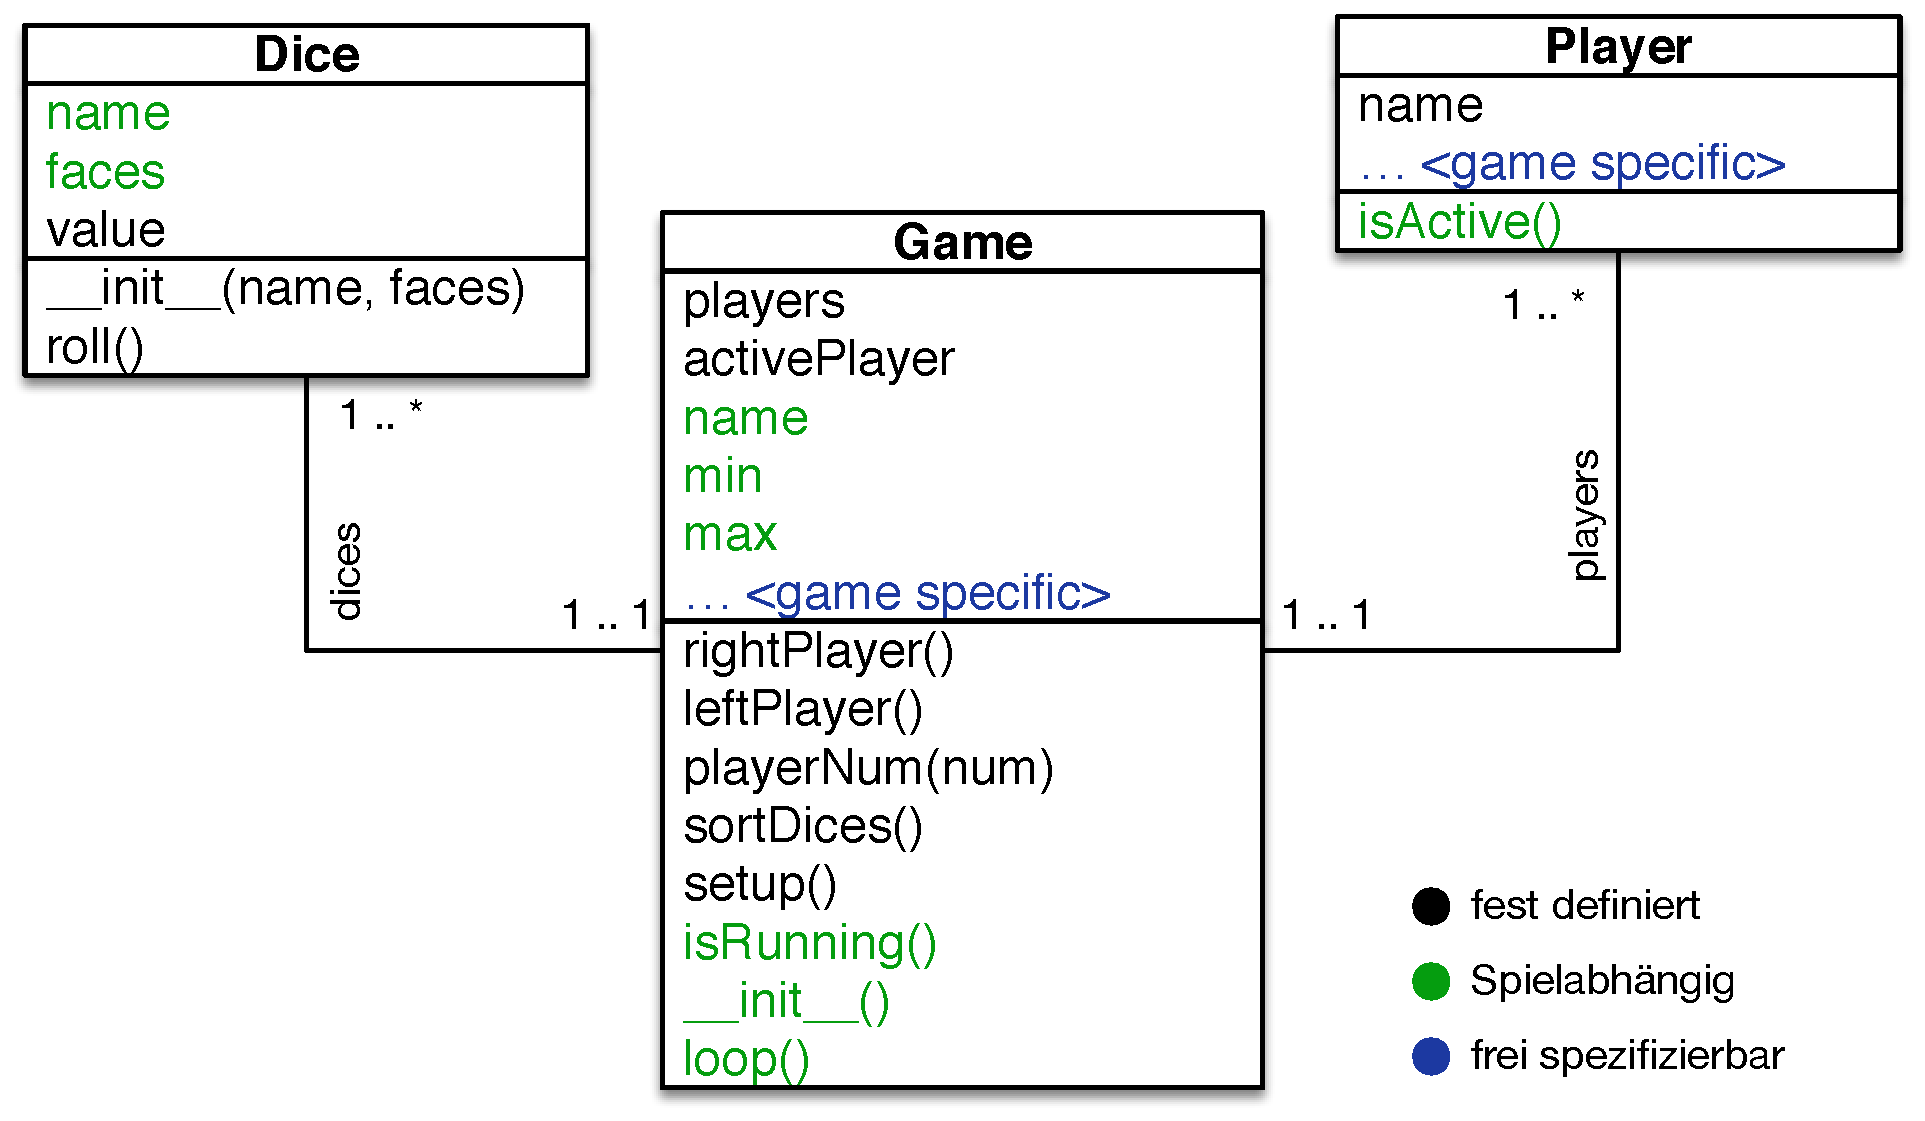
\includegraphics[width=0.8\textwidth]{Python-UML.pdf}
    	\caption{Klassendesign des Python Frameworks}
    	\label{python-uml}
    \end{figure}

    Die domänenspezifischen Methoden können direkt aus der Sprache verwendet werden und entsprechen den verwendbaren Anweisungen (\texttt{würfelt mit <würfeln>}).

\section{Interne Datenrepräsentation}
\label{sec:interne_datenreprasentation}
    Wie in den obigen Abschnitten erwähnt, werden für die Implementierung Konstrukte unserer Zielsprache verwendet. Der objektorientierte Ansatz von \dg zeigt sich hier in der Umsetzung in Klassen für Spieler, Würfel und das Spiel selbst. Bei der Übersetzung eines Spiels werden Teile der gegebenen Klassen durch die vom Spielentwickler spezifizierten Eigenschaften des Spiels ergänzt. Beispiel dafür sind die Spieler, denen durch den Spielentwickler neuen Felder hinzugefügt werden können.Die Würfelklasse hingegen ist nicht erweiterbar, sondern wird nur durch die Implementierung der Spielklassen verschieden initialisiert.

    Die Spielklasse enthält die Initialisierung und den Ablauf des Spiels und ist die zentrale Klasse. Die Klasse enthält einige generische Methoden, die nicht individualisierbar sind und in der Sprache zur Verfügung stehen (\texttt{leftPlayer()}, \texttt{rightPlayer()}, \texttt{sortDices()}, ...). In Kontrast dazu bildet die \texttt{loop()}-Methode den Spielablauf ab und wird vom Entwickler frei definiert.

\section{Compilerimplementierungen}
\label{sec:compilerimplementierungen}
	Da die Implementierung recht umfangreich ist kann sie hier nicht vollständig sondern lediglich beispielhaft angegeben werden.

	\dg wurde so konzipiert, dass alle domänenspezifischen Konzepte, wie sie oben beschrieben sind, direkt abgebildet werden können. Auch in der Pythonumsetzung wurde versucht dies beizubehalten und die Konzepte von \dg soweit wie möglich direkt in Python umzusetzen. Grundoperationen wie \texttt{+, -, *, größer, kleiner, gleich, ...} wurden direkt in ihren entsprechenden Pythonoperatoren umgesetzt, woraus eine lazy evaluation arithmetischer Operationen folgt. Gleiches gilt für die Zuweisung. Diese kann in \dg zwar syntaktisch unterschiedlich ausgedrückt werden (\texttt{<Variable> ist <Ausdruck>} oder \texttt{setze <Variable> auf <Ausdruck>}), in Python wird daraus aber immer eine einfache Zuweisung.

	Desweiteren wurden einige Abstraktionen vorgenommen, um die Paradigmen aus der Domäne umzusetzen. Als Beispiel sei folgender Code gegeben:
\begin{lstlisting}
wenn würfel A gleich 2 ...
\end{lstlisting}
	In konventionellen Programmiersprachen wäre diese Operation nicht ohne Weiteres möglich, da ein Vergleich zwischen einem selbst definierten Objekt und einer Zahl zunächst nicht definiert ist. Im Bezug auf die Domäne ist dieser Ausdruck jedoch sinnvoll, da damit implizit gemeint ist, dass der gewürfelte Wert, also eine Zahl mit einer anderen verglichen werden soll. Diesen Umstand nutzen wir, sodass ein logischer Vergleich oder eine arithmetische Operation mit Würfeln immer als Operation auf dem entsprechenden gewürfelten Wert zu verstehen ist. Im Code sieht das wie folgt aus:
\begin{lstlisting}
if [dice for dice in self.dices if dice.name == 'A'].value == 2 ...
\end{lstlisting}
	Diese Idee wurde versucht so weit wie möglich umzusetzen. Sie findet sich beispielsweise in der Referenzierung des nächsten Spielers wieder. Hier genügt es in \dg zum Beispiel das Schlüsselwort \texttt{linker spieler} zu verwenden. Diese Abstraktion wurde in Python so umgesetzt, dass der Index der Liste, in dem Spieler gespeichert sind, um eins dekrementiert wird.

	Weiterhin soll hier auf die Implementierung der Methode \texttt{isRunning()} eingegangen werden. Diese repräsentiert die Bedingung, die der Entwickler festlegen kann. Sie bestimmt, ob ein Spiel noch läuft oder nicht. Beispielsweise kann ein Spiel nach $n$ Runden zu Ende sein.
\begin{lstlisting}[label={lst:ODD}]
ODD wird so gespielt:

das spiel hat den wert RUNDEN ist 5.
...
das spiel läuft solange RUNDEN größer 0.
...
\end{lstlisting}
	Im oberen Listing wird beispielsweise die globale Variable \texttt{RUNDEN} definiert und als Bedingung festgelegt, dass ein Spiel solange läuft, solange \texttt{RUNDEN größer 5} gilt. Das heißt das Spiel läuft fünf Runden. Im kompilierten Pythoncode sieht das wie folgt aus:
\begin{lstlisting}[language=Python]
def isRunning(self): return (self.RUNDEN > 0)
\end{lstlisting}
	Diese Methode hat eine weitere Besonderheit. Wird keine Bedingung festgelegt, weil ein Spiel beispielsweise kein deterministisches Ende hat, sondern von Fall zu Fall unterschiedlich ist, hat die Funktion einen Standardfall, bei dem immer \texttt{true} zurückgegeben wird. In diesem Fall muss sich der Entwickler aber selbst darum kümmern, das Spiel mit dem Schlüsselwort \texttt{das spiel ist zu ende.} zu beenden. Methoden dieser Art, also die gegeben sein müssen, aber vom Nutzer gefüllt werden können, gibt es noch weitere, beispielsweise die Funktion \texttt{isActive()}, die nach einer von Entwickler definierten Bedingung entscheidet, ob ein Spieler aktiv ist oder nicht.

\section{Erfüllung der geforderten Sprachqualitäten}
\label{sec:erfullung_der_geforderten_sprachqualitaten}
	Zentrale Qualität der Sprache ist die Einfachheit und die daraus folgende Robustheit durch Einschränkung der Mächtigkeit. Ein Beispiel für die Erfüllung dieses Kriteriums liegt in der automatischen Interpretation von Würfelreferenzen. Wird ein Würfel in einer arithmetischen Operation verwendet, so wird stets der aktuell angezeigte Wert referenziert. Dem Spieleentwickler ist es damit nicht möglich einen Würfel mit einer Zahl zu addieren, er adressiert in diesem Fall automatisch das Ergebnis.

	Ein Beispiel, in dem die geforderte Robustheit noch fehlt, ist die Verwendung von \texttt{für}-Schleifen. Der Nutzer muss hier einen Bezeichner definieren, auf den er im Schleifenrumpf zugreifen kann. Denkbar wäre eine vereinfachte Version, in der Variablen des iterierten Objektes und die des globalen Scopes zusammenliegen und direkt verwendet werden können. Diese Variante würde die Syntax vereinfachen. In dieser Version unserer Sprache wurde zu Gunsten einer einfacheren Implementierung für eine konventionelle For-Schleife entschieden.

\section{Mögliche Erweiterungen}
\label{sec:mogliche_erweiterungen}
	Im Laufe der Entwicklung von \dg wurde Konzepte entwickelt und diskutiert, die es nicht in die Implementierung geschafft haben oder sich im Nachhinein als falsch oder unzulänglich erwiesen haben.

	Zunächst wäre da die Implementierung des Frameworks zu nennen. Hier gibt es in der aktuellen Version konkrete Klassen, die dynamisch mit den von Nutzer spezifizierten Elementen gefüllt werden. Da mit Python jedoch eine objektorientierte Sprache verwendet wird, wäre es sinnvoller abstrakte Basisklassen von Spielern, Würfeln und dem Spiel zur Verfügung zu stellen, von denen eine implementierte Klasse angelegt wird, die von der entsprechenden Klasse erbt. Somit hätte man auch die Objektorientiertheit, die in \dg teilweise inhärent gegeben ist auch auf die Implementierung angewandt. Eine Möglichkeit der Modularität wäre somit gegeben, die in der aktuellen Version jedoch verloren geht.

	Außerdem hat \dg einige syntaktische Konstrukte, die von der Entscheidung, die Sprache so intuitiv und einfach wie möglich zu gestalten, abweichen. Zu erwähnen ist die Adressierung und Referenzierung von Würfeln. Im aktuellen Zustand haben Würfel Namen, die der Entwickler vorgeben muss. Will man nun den Wert dieses Würfels haben, kann das auf zwei Arten geschehen. Entweder über den Namen oder über einen Index. Dieser Index wird allerdings erst logisch sinnvoll, wenn eine Sortierung der Würfel stattgefunden hat. Außerdem scheint die Adressierung über den Namen nicht aus der Domäne hervorzugehen, da man Würfeln normalerweise keine Namen gibt. Um das zu erleichtern oder intuitiver zu gestalten, könnten beispielsweise neue syntatkische Konstrukte wie \emph{Pasch} oder \emph{Straße} eingeführt werden, die die Überprüfung dieser Ereignisse vereinfacht.

	Schließlich waren zu Beginn Konstrukte geplant, die es dem Entwickler ermöglichen eigene Nutzerinteraktion zu definieren, beispielsweise Ausgaben auf der Kommandozeile oder die Möglichkeit auf Ereignisse dynamisch zu reagieren und nicht nur nach fest definierten Regeln vorzugehen. Der Fokus lag jedoch zunächst auf den Konzepten, die von der Domäne gegeben sind und die Sprache möglichst einfach zu gestalten. Daher wurde dieser Punkt mit einer niedrigen Priorität hinten angestellt und ist in der aktuellen Referenzimplementierung nicht enthalten.